%%%%%%%%%%%%%%%%%%%%%%%%%%%%%%%%%%%%%%%%%%%%%%%%%%%%%%%%%%%%%%%%%%%%%%
% LaTeX Example: Project Report
%
% Source: http://www.howtotex.com
%
% Feel free to distribute this example, but please keep the referral
% to howtotex.com
% Date: March 2011 
% 
%%%%%%%%%%%%%%%%%%%%%%%%%%%%%%%%%%%%%%%%%%%%%%%%%%%%%%%%%%%%%%%%%%%%%%
% How to use writeLaTeX: 
%
% You edit the source code here on the left, and the preview on the
% right shows you the result within a few seconds.
%
% Bookmark this page and share the URL with your co-authors. They can
% edit at the same time!
%
% You can upload figures, bibliographies, custom classes and
% styles using the files menu.
%
% If you're new to LaTeX, the wikibook is a great place to start:
% http://en.wikibooks.org/wiki/LaTeX
%
%%%%%%%%%%%%%%%%%%%%%%%%%%%%%%%%%%%%%%%%%%%%%%%%%%%%%%%%%%%%%%%%%%%%%%
% Edit the title below to update the display in My Documents
%\title{Project Report}
%
%%% Preamble
\documentclass[paper=a4, fontsize=11pt]{scrartcl}
\usepackage[T1]{fontenc}
\usepackage{fourier}
\usepackage{float}
\usepackage[english]{babel}															% English language/hyphenation
\usepackage{needspace}
\usepackage[protrusion=true,expansion=true]{microtype}	
\usepackage{amsmath,amsfonts,amsthm} % Math packages
\usepackage[pdftex]{graphicx}	
\usepackage{parskip} % Sets space between paragraphs
\usepackage{url}
\usepackage{hyperref}
\usepackage{lineno}
\usepackage{color, soul}
\usepackage{graphicx}
\graphicspath{ {./images/} }

% Adds colours to links
\hypersetup{
    colorlinks=true,
    linkcolor=magenta, % makes links to equations, figs, etc magenta
    urlcolor=blue, % makes url links blue
    citecolor = red % makes citation links red
}

\newcommand{\appropto}{\mathrel{\vcenter{
  \offinterlineskip\halign{\hfil$##$\cr
    \propto\cr\noalign{\kern2pt}\sim\cr\noalign{\kern-2pt}}}}}

%%% Custom sectioning
\usepackage{sectsty}
\allsectionsfont{\centering \normalfont\scshape}


%%% Custom headers/footers (fancyhdr package)
\usepackage{fancyhdr}
\pagestyle{fancyplain}
\fancyhead{}											% No page header
\fancyfoot[L]{}											% Empty 
\fancyfoot[C]{}											% Empty
\fancyfoot[R]{\thepage}									% Pagenumbering
\renewcommand{\headrulewidth}{0pt}			% Remove header underlines
\renewcommand{\footrulewidth}{0pt}				% Remove footer underlines
\setlength{\headheight}{13.6pt}


%%% Equation and float numbering
\numberwithin{equation}{section}		% Equationnumbering: section.eq#
%\numberwithin{figure}{section}			% Figurenumbering: section.fig#
\numberwithin{table}{section}				% Tablenumbering: section.tab#
\usepackage{gensymb}
\usepackage{relsize}
%%% Maketitle metadata
\newcommand{\horrule}[1]{\rule{\linewidth}{#1}} 	% Horizontal rule


%% To use line numbers 
%\linenumbers

%% create a title page
\title{
		%\vspace{-1in} 	
		\usefont{OT1}{bch}{b}{n}
		\normalfont \normalsize \textsc{Queen's University} \\ [25pt]
		\horrule{0.5pt} \\[0.4cm]
		\huge Humpback Whale Identification Report \\
		\horrule{2pt} \\[0.5cm]
}
\author{
    \normalfont 
      CISC 867 - Deep Learning Project \\
    \normalfont
    Group Members: \\ 
    \normalsize
    Emily Medema (20340337) \\ 
    \normalsize
    Stephen McKeon (20379475) \\ 
    \normalsize
    Flourish Adebayo (20312488) \\
    November 28, 2022 \\ [3pt]}
\date{\vspace{-5ex}}


%%% Begin document
\usepackage{graphicx}
\graphicspath{ {./images/} }
\begin{document}
%% remove the page number on the title page 
\pagenumbering{gobble}
%% need this line to add the title page you just created 
\maketitle
\needspace{15em}
%% the section command gives a new section with the given header. 
\section*{Abstract}\label{sec: abstract}

This report will go into the process of identifying humpback whales based on their fluke using deep learning techniques. We will use a CNN, Transfer Learning, and a SVM and compare their results to find the most effective model for the identification of individual humpback whales. Our architecture can be seen in Figure \ref{fig:archabstract}. CNN and Transfer learning predictably perform well, but due overfitting in the CNN model, Transfer Learning is the better model.

%% go to a new page 
\newpage 
%% start the page numbering again 
\pagenumbering{arabic}

\section*{Introduction}\label{sec: intro}
%Define and motivate the problem, discuss background material or related work, and briefly summarize your approach.
The Humpback Whale is a species of baleen whale. It has a distinctive body shape with long pectoral fins and a knobbly head. They are known for their infringing and surface behaviour making them popular with whale watchers\cite{kareiva2006whales}. Despite this popularity, at the beginning of the 20th century whale populations dropped but did increase briefly in the mid-20th century due to the creation of the international whaling committee in 1946\cite{henderson2022behavior}. Nonetheless, whale populations are still fluctuating and requiring protection. To better understand the preservation effort, researchers utilize photo surveillance mechanisms to understand marine activities. Researchers utilize a variety of features of whales such as the shape, markings, and tail length to help identify the type of whale they are analyzing \cite{JaisakthiS.M.2017Awms}. In fact, many scientific studies are utilizing photography as a method of monitoring their projects, in this case it is usually pictures of whale fins. This usually results in a scientist having to analyze these images themselves, which can take many hours and a lot of technical knowledge \cite{JaisakthiS.M.2017Awms}. However, we can now use image classification models to perform these same tasks in a lot less time with comparable accuracy \cite{JaisakthiS.M.2017Awms}.

Image classification is a booming area of interest in the Computer Vision and Machine Learning fields. Due to the rapid increase of image sharing after the popularity of social media and personal cameras (and later smartphones) \cite{jain2000statistical}, there are a surplus of images to classify and analyze on the internet. There are different algorithms for image classification, the most common of which are deep learning and machine learning. Different models have distinct results in different problem areas, with image classification traditionally using traditional deep learning and machine learning algorithms for its numerous advantages. 

In fact, Deep Neural Networks (DNN) is growing exponentially in the field of Machine Learning (ML). Of the many DNN structures, Convolutional Neural Networks (CNN) are presently the main tool used for image analysis and classification purposes \cite{jain2000statistical}. Comparison and evaluation of images using classification algorithms based on traditional machine learning and deep learning are of great significance for selecting algorithms to classify pictures. 

The Humpback Whale Identification Challenge is a Kaggle Competition \cite{WhateIdentifcationChallengeKaggle} created to aid whale conservation efforts with the creation of an algorithm to identify individual whales in images. After centuries of intense whaling, recovering whale populations still have a hard time adapting to warming oceans and struggle to compete every day with the industrial fishing industry for food. Scientists use photo surveillance systems to monitor whale activity and can use the shape of whales’ tails and unique markings to identify particular whales and analyze their movements \cite{JaisakthiS.M.2017Awms}.

%% TODO: refined
Data obtained from this challenge was used to compare and analyze popular image classification machine learning models. In this project, we compare a Convolutional Neural Network (CNN) with transfer learning, as well as classical machine learning model - an SVM - to detect the identity of humpback whales in the picture.


\section{Background}\label{sec: background}

Despite lacking predators, whales have continued to be endangered. As whales play a large role within the ocean's ecosystem, conservation efforts have been consistent over the years in order to ensure a stable food chain. Part of these conservation efforts is the tracking of whales to know the health and status of their species by marine biologists. This is mainly done through aerial surveillance and manual identification, which is a very time consuming process \cite{JaisakthiS.M.2017Awms}. As whale fins are identifiable features for individual whales, biologists are able to develop conservation strategies by observing individual whale and entire whale species behaviours. This can take a lot of time and resources. Automating this process with a machine learning model to identify unique whales will alleviate this stress and allow for more time to develop better strategies for the continued survival of whales.

As machine and deep learning continued to develop, we began to see the potential for use. In the paper by He et al. \cite{he2016deep}, Residual Network, commonly referred to as ResNet, was first introduced. It applied residual sections to estimate a denoised image which achieves a classification accuracy comparable to that of a human. In 2006 Zhang et al. published a paper where a SVM KNN was utilized - an improved version of the traditional KNN classifier \cite{zhang2006svm}. It converts the distance of K neighbours and applies a multi-class Support Vector Machine. We began to see the use of these models in 2017 with the paper “Towards automated visual monitoring of individual gorillas in the wild” in which the authors used different techniques for automating the identification of animals employing computer vision \cite{brust2017towards}. They gave the context and evaluation of the system for an automatic interpretation of sightings of individual western lowland gorillas using SVM which gave an accuracy of 62.40\%. We see the use of machine learning for animal identification again in the paper by Shukla et al. in which a hybrid system was built to assist in the re-identification of tigers \cite{shukla2019hybrid}. The authors used handcrafted features from pictures to detect animals based on patterns using cosine similarity which gave an accuracy of 89.10\%. We began to see the use of deep learning models in 2018 when Bergamini et al.  stated that the use of deep learning methods is suitable for identification and yielded increased accuracy and overall performance of detection \cite{bergamini2018multi}. Specifically, the authors used a multi-view embedding model for cattle re-identification with a KNN classifier which gave an accuracy of 81.70\%. Freytag et al. used log-Euclidean CNNs for predicting identities and attributes of primates which gave an accuracy of 84.50\%  \cite{freytag2016chimpanzee}. As we can see, the history of utilizing machine and deep learning models for animal identification is long and varied, thus it makes sense that we now apply it to Humpback Whale Identification.

Over the years, a lot of research has been done in this field. There have been multiple Kaggle competitions and there are a multitude of approaches to this problem. While there have been some studies on the application of transfer learning augmenting deep learning and classical machine learning models \cite{YuanHongchun2020AAIC}, it's effectiveness in this particular problem space compared to a classical machine learning model, such as SVM, as well as a deep learning model itself (without transfer learning) can be further explored.

\section{Data}\label{sec: data}

The \href{https://www.kaggle.com/competitions/humpback-whale-identification/overview}{Humpback Whale Identification} competition \cite{WhateIdentifcationChallengeKaggle} on Kaggle contains thousands of images of humpback whale flukes - 25,361 files (76.11\% of dataset) for training and a further 7,960 (23.89\% of dataset) for testing. Individual whales have been identified by researchers and given an identification (Id). The challenge is to predict the whale Id of images in the test set. This is particularly challenging for two primary reasons:
\begin{itemize}
  \item The heterogeneity of the data. Images drastically vary in size. Some are greyscale, others are in colour. Some whale flukes are pointing towards the sky, others are not. Normalizing the data will be extremely important and is discussed in \autoref{subsec:Preprocessing}.
  \item Imbalance in the dataset. There is a relatively small dataset compared to the 5,000 unique whale Ids present in the data. Only 227 whales are represented in the dataset more than 10 times while over 2,000 whales are represented by only a single sample, as shown in \autoref{fig:ID_Occ}. To compensate for this we will be utilizing data augmentation as discussed later in \autoref{subsec:Augmentation}.
\end{itemize}

\begin{figure}[H]
    \centering
    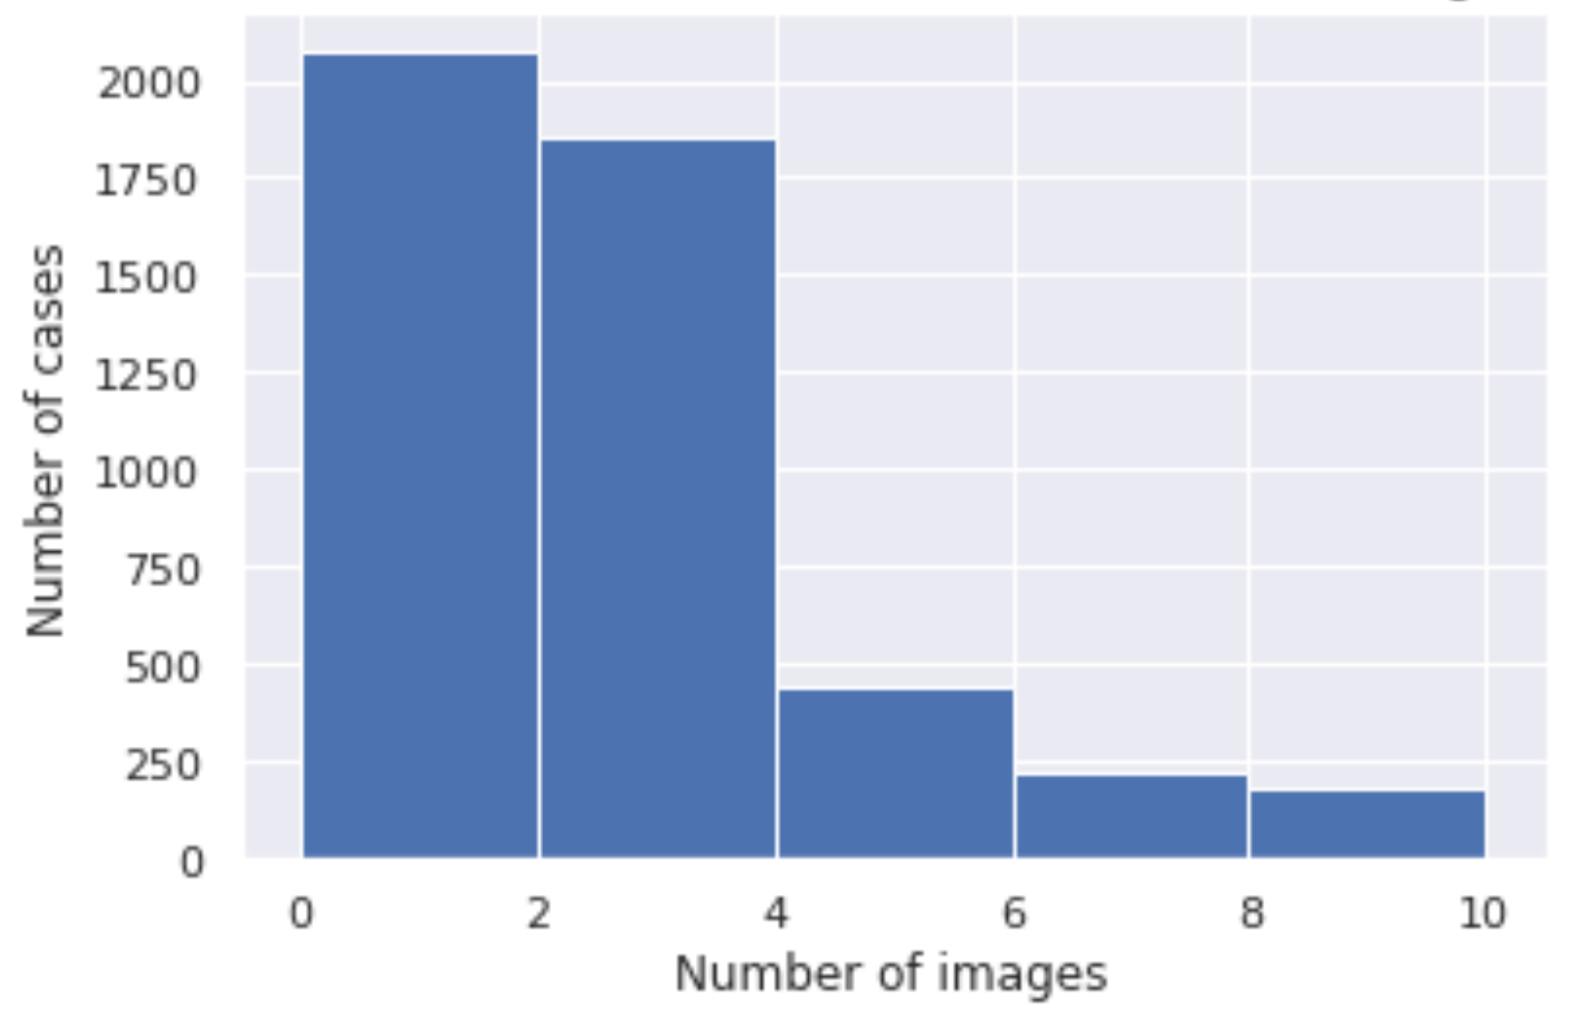
\includegraphics[width=0.5\textwidth]{ID_Occurences.png}
    \caption{Number of cases for various numbers of whale images}
    \label{fig:ID_Occ}
\end{figure}

\section{Methodology}\label{sec: meth}

%Details of the approach: Include any formulas, pseudocode, diagrams -- anything that is necessary to clearly explain your system and what you have done. If possible, illustrate the intermediate stages of your approach with results images.

%TODO: finish the machine learning model section

In order to identify whales by their fluke, data prepossessing was conducted to remove noise and crop to show only the fluke. Due to the sparse number of images of the same whale, we performed data augmentation by flipping, rotating and scaling of the images as needed within the training of the models. This allows us to develop a more accurate, robust model and reduce overfitting. We then attempt to identify the whale via a developed CNN model, transfer learning, and a SVM. The architecture of the Humpback whales identification is shown in \autoref{fig:Architecture}. 

The various steps involved in  identifying Humpback whales are:
\begin{itemize}
    \item Preprocessing the data
    \item Augmentation of the data
    \item Classification with CNN
    \item Classification with Transfer Learning
    \item Classification with SVM
    \item Comparison of Results
\end{itemize}

\begin{figure}[H]
    \centering
    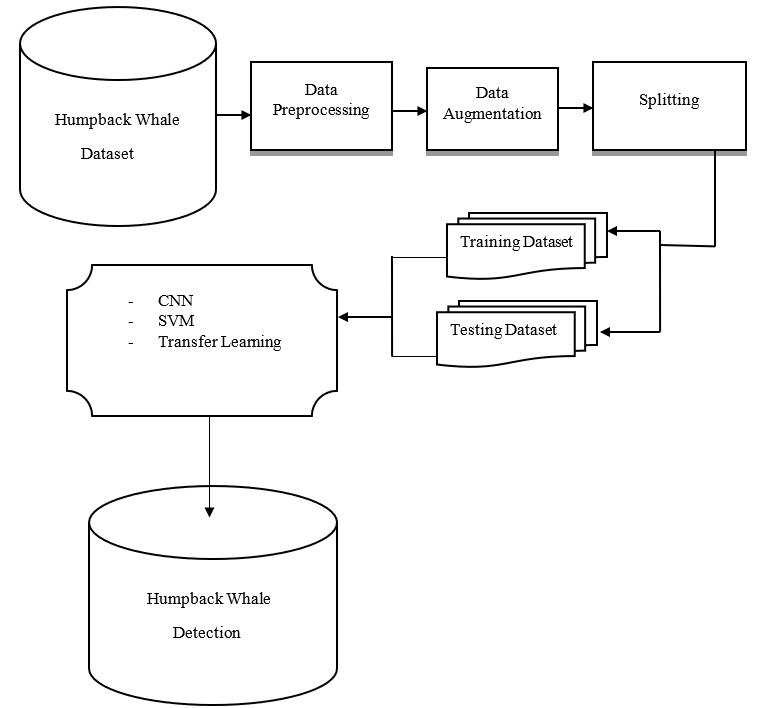
\includegraphics[width=0.6\textwidth]{Architecture.PNG}
    \caption{Architecture Diagram of Humpback Whale Identification }
    \label{fig:Architecture}
\end{figure}

\subsection{Data Preprocessing}\label{subsec:Preprocessing}

The first step for the preprocessing of the data was to crop as much noise from the images as possible, such as the background in the images. While many of the whale pictures in the dataset were already cropped tightly around the whale fluke, in some images the whale fluke occupied only a small area of the picture. Zooming onto the relevant part of the picture provides greater accuracy to a classification model. 

A couple of months before this competition, a playground version of the same competition was hosted on Kaggle, but, as it was noted by the competition hosts, the real version featured even more data and cleaner labels. We were able to leverage the pre-trained weights from a CNN model from the playground version of the competition that identified the coordinates specifying a bounding box around the fluke of the whale in each image \cite{FlukeDetection}. The CNN model used to determine the proper bounding box of the whale fluke in each image was quite complex, as shown in \autoref{tab:table1}. Leveraging the weights from the trained model saved a lot of time.

\begin{table}[h!]
  \begin{center}
    \caption{CNN - Bounding Box Model}
    \label{tab:table1}
    \begin{tabular}{l|c|r} % <-- Alignments: 1st column left, 2nd middle and 3rd right, with vertical lines in between
      \textbf{Layer} & \textbf{Output Shape} & \textbf{Params}\\
      \hline
      InputLayer & (128, 128, 1) & 0\\
      Conv2D & (128, 128, 64) & 5248\\
      Conv2D & (128, 128, 64) & 36928\\
      BatchNormalization & (128, 128, 64) & 256\\
      Conv2D & (64, 64, 64) & 16448\\
      Conv2D & (64, 64, 64) & 36928\\
      Conv2D & (64, 64, 64) & 36928\\
      BatchNormalization & (64, 64, 64) & 256\\
      Conv2D & (32, 32, 64) & 16448\\
      Conv2D & (32, 32, 64) & 36928\\
      Conv2D & (32, 32, 64) & 36928\\
      BatchNormalization & (32, 32, 64) & 256\\
      Conv2D & (16, 16, 64) & 16448\\
      Conv2D & (16, 16, 64) & 36928\\
      Conv2D & (16, 16, 64) & 36928\\
      BatchNormalization & (16, 16, 64) & 256\\
      Conv2D & (8, 8, 64) & 16448\\
      Conv2D & (8, 8, 64) & 36928\\
      Conv2D & (8, 8, 64) & 36928\\
      BatchNormalization & (8, 8, 64) & 256\\
      Conv2D & (4, 4, 64) & 16448\\
      Conv2D & (4, 4, 64) & 36928\\
      Conv2D & (4, 4, 64) & 36928\\
      BatchNormalization & (4, 4, 64) & 256\\
      MaxPooling2D\_1 & (4, 1, 64) & 0\\
      MaxPooling2D\_2 & (1, 4, 64) & 0\\
      Flatten\_1 & (256) & 0\\
      Flatten\_2 & (256) & 0\\
      Dense\_1 & (16) & 4112\\
      Dense\_2 & (16) & 4112\\
      Concatenate & (32) & 0\\
      Dense & (4) & 132\\
    \end{tabular}
      \small
      \item Trainable params: 502,820
  \end{center}
\end{table}

By describing the same neural network and loading the pre-trained weights, the training dataset could then be passed to the model and evaluated to obtain the coordinates for bounding boxes around the whales' flukes. These coordinates can then be used to visualize the bounding box region, as shown in \autoref{fig:fig1}.

\begin{figure}[h]
    \centering
    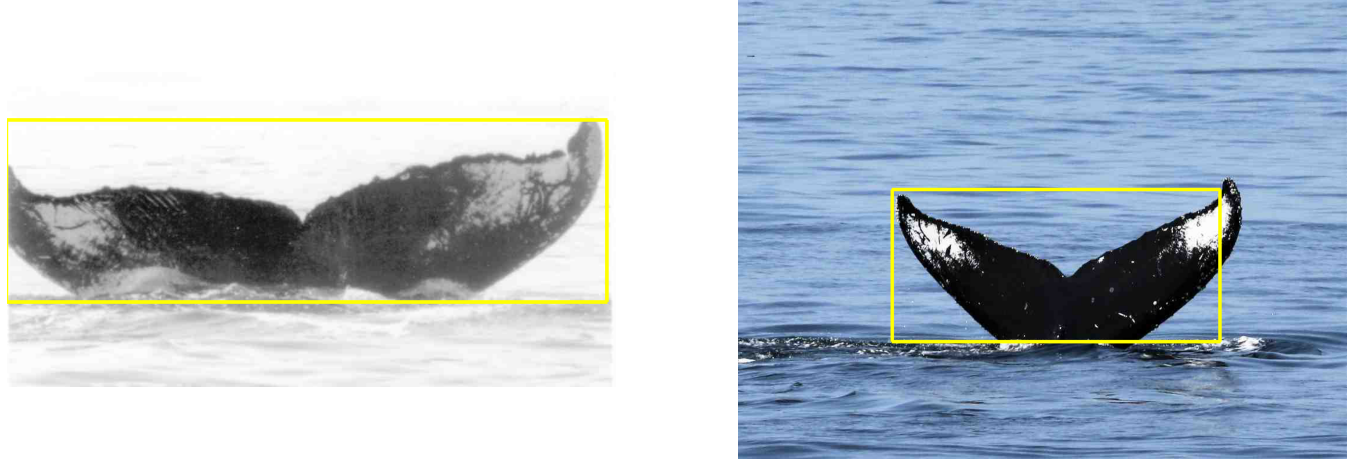
\includegraphics[width=0.5\textwidth]{BoundingBoxExample.png}
    \caption{Coordinates for Bounding Box overlayed on the corresponding images}
    \label{fig:fig1}
\end{figure}

\begin{figure}[h]
    \centering
    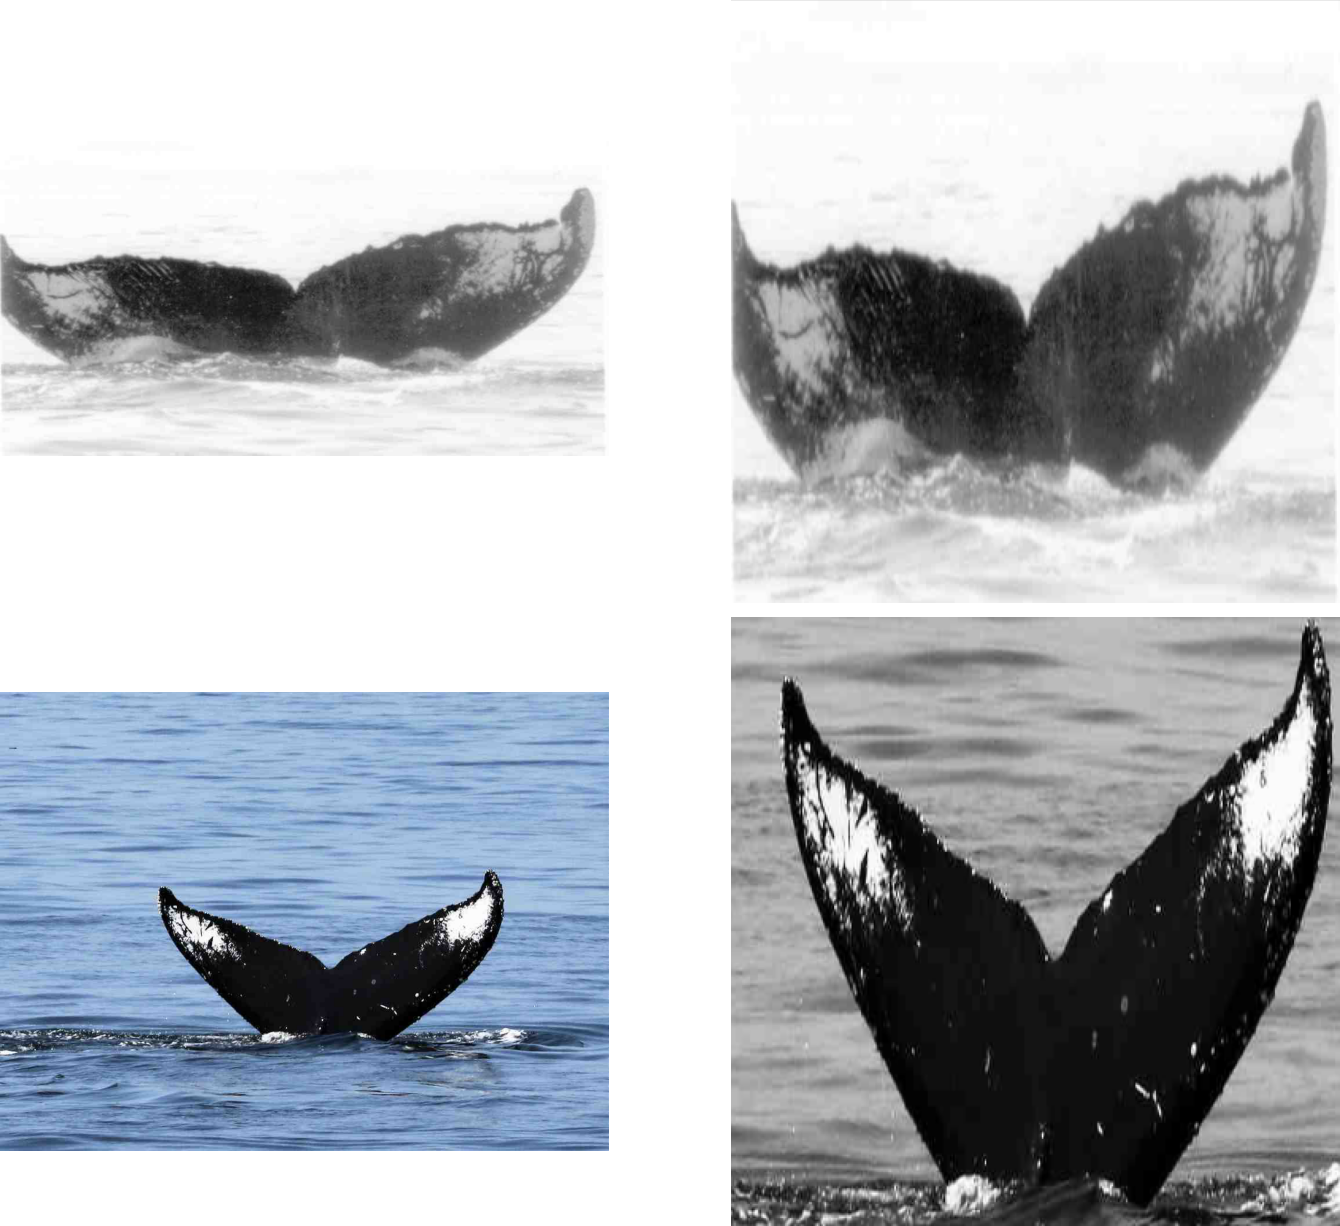
\includegraphics[width=0.5\textwidth]{ProcessedImages.png}
    \caption{Original images (left) and their corresponding processed images (right)}
    \label{fig:fig2}
\end{figure}

As you can see, the resulting bounding boxes are not perfect. This can be resolved by extending the region described by the bounding box before cropping the image. The idea is that clipping the edges of the fluke is more harmful than the noise obtained by fitting it exactly, thus an increased margin is preferred. Through trial and error, we determined that extending the crop region by 8\% was sufficient to ensure the entire fluke was captured. This is shown to have succeeded when comparing the coloured image from \autoref{fig:fig1} with the output from \autoref{fig:fig2}.

As shown in the previous \autoref{fig:fig1}, some of the images in the dataset are greyscale and some are colour. In order to standardize the data and ensure our model does not learn any colour-only or greyscale-only specific features, we converted all images to greyscale.

An affine transformation is a geometric transformation that preserves lines and parallelism - but not necessarily distances and angles. The final step for data preprocessing was to take the cropped area from the previous step and transform it to a uniform size for use as input to a neural network - in our case, 384x384x1 (only one channel for black and white). The resulting changes after cropping, converting to greyscale, and applying the affine transformation to the images from the previous figure are shown in \autoref{fig:fig2}. With these changes, the data is normalized so that there is as little variation as possible within the dataset aside from the differences between each whale's flukes.

One final manipulation of the data was the removal of particular samples. In the training dataset, numerous samples were classified as "new\_whale" as opposed to the identification number associated with a particular individual whale. The image features associated with the various "new\_whale" samples, however, do not share any logical overlap. They are different individuals. While these samples would be useful in the testing phase of our model, they do not contribute to proper learning during training; hence, they were removed.

\subsection{Data Augmentation}\label{subsec:Augmentation}
Due to the nature of the data - that is, certain classes with numerous instances and many classes with only one instance - we will have to heavily augment the data. The intent is to augment the data by a combination of flipping, rotating, shearing, zooming, shifting, and random brightness. The intent is to put an emphasis on creating more samples for classes that are under-represented, so these will be augmented with every possible combination of our augmentation strategies, while over-represented classes will remain untouched. 

During the training of our various models, it was determined that performing additional data augmentation on the smaller dataset was decreasing the performance of the Transfer Learning model. Specifically, zooming, shearing, shifting and rotating seem to \textbf{reduce} the model's efficacy. This is likely because the data was already preprocessed to center and reduce noise by zooming in on just the fluke of the whale. That effort was erased by these augmentation techniques. By removing those additional techniques, the models trained faster and performed better. We continued to utilize flipping and random brightness, however, as these techniques did not hinder the training process. However, unlike the Transfer Learning model, data augmentation improved the CNN model, including zooming, shearing, shifting, and rotating. Nonetheless, in order to ensure fair comparison the CNN model utilized the same augmentation as the Transfer Learning model.

\subsection{Model Training and Testing}

\subsubsection{Model 1}

The first model we will utilize for classification is a CNN using the python library Keras. Before we could train the model itself, we had to transform the data into a form that could be utilized for classification, as discussed in  \autoref{subsec:Preprocessing}. After reading in the data, we separated the X and Y (i.e., input and output variables), the image name and the whale id respectively. After some preliminary data analysis of the data, we drop the 'new\_whale' classification as those are whales with only one image, which is not conducive for the initial training of a model to identify matching whales. Similarly, due to the processing power available to us, we restrict the whales to only those with five or more images. We then read in the images for each image name as an array. We then hot-encoded our response variable which will help with classifying the output of the CNN. Once the transformation of the data was done, we began to build our model.

The basics of our model are two convolutional layers with the padding of the model to "same", a max-pooling layer, and batch-normalization. This is followed by another round of two convolutional layers with "same" padding, a max-pooling layer, and dropout. We then follow it again with two more convolutional layers with "same" padding, another max-pooling layer and batch-normalization. After which, we start the fully-connected layer for classification by flattening the input and two dense layers with a batch-normalization in between. We decided to utilize max-pooling as this means our output shape follows the following equation: $output\_shape = math.floor((input_shape - 1) / strides) + 1$. We also used batch-normalization and Dropout in an attempt to prevent over-fitting. The Adam optimizer was used to optimize the gradient descent of our model.

In order to determine if this model architecture would work for our data, we trained it with 10\% of the training data. If the model overfit onto this subset of the data, that means the model would most likely accurately work on the entire dataset.

After running the model on the subset of data, we received an overfitting of the data as seen in Figure \ref{fig:cnn_acc_10p} and Figure \ref{fig:cnn_loss_10p} with extremely high accuracy and extremely low loss.

\begin{figure}[h]
    \centering
    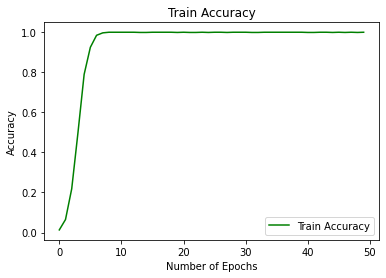
\includegraphics[width=0.5\textwidth]{training_cnn_acc_10p.png}
    \caption{Training Accuracy on 10\% of Training Data}
    \label{fig:cnn_acc_10p}
\end{figure}

\begin{figure}[h]
    \centering
    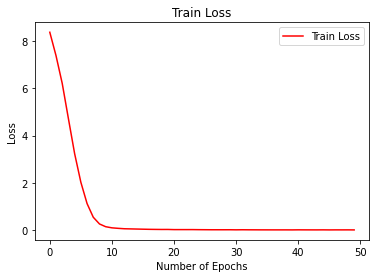
\includegraphics[width=0.5\textwidth]{training_10p_loss.png}
    \caption{Training Loss on 10\% of Training Data}
    \label{fig:cnn_loss_10p}
\end{figure}

Now that we know that a CNN model like this works for our data, we trained it on a larger subset of the data, specifically all data where there are 5 or more images of a specific whale. We then split the data into training and validation sets. Fitting the model as described above onto this data resulted in an overfit onto the training data. We now began tuning the model to reduce the overfit and ensure we have the best hyper-parameters selected. We first tested 'relu' activation or 'tanh' activation and different number of units for the Dense layers in the classification section of the model. Through this we determined that 'relu' was the best activation function for our model. We then began to tune for less overfit by testing different rates of dropout and adding more dropout layers to the model. Through this we discovered that 0.25 for the second and third dropout layer creates the best result. Nonetheless, it was still overfitting on the training data so we began to test adding in l2 regularization. We found the best rates of l2 for less overfit, however, it was still overfit. We then introduced data augmentation via running ImageDataGenerator on 'x\_train'. Through this method, we received the best result so far with a high training accuracy and a higher validation accuracy as seen in Figure \ref{fig:cnn_acc_da} and a relatively high top-5 accuracy for both training and validation as seen in Figure \ref{fig:top5cnn}. It also has a lower loss as seen in Figure \ref{fig:cnn_loss_da}. It is still overfit, but it would require more processing power and images for us to get a better result than is available to us at this time.

\begin{figure}[!h]
    \centering
    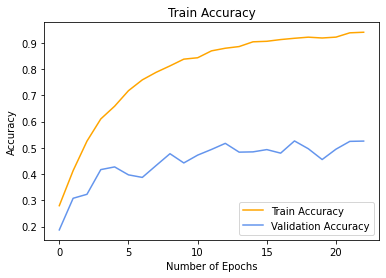
\includegraphics[width=0.5\textwidth]{images/cnn_acc_da_l2.png}
    \caption{Tuned CNN Training Accuracy with Data Augmentation}
    \label{fig:cnn_acc_da}
\end{figure}

\begin{figure}[!h]
    \centering
    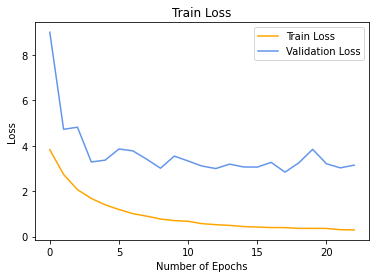
\includegraphics[width=0.5\textwidth]{images/cnn_loss_da_l2.png}
    \caption{Tuned CNN Training Loss with Data Augmentation}
    \label{fig:cnn_loss_da}
\end{figure}

\begin{figure}[!h]
    \centering
    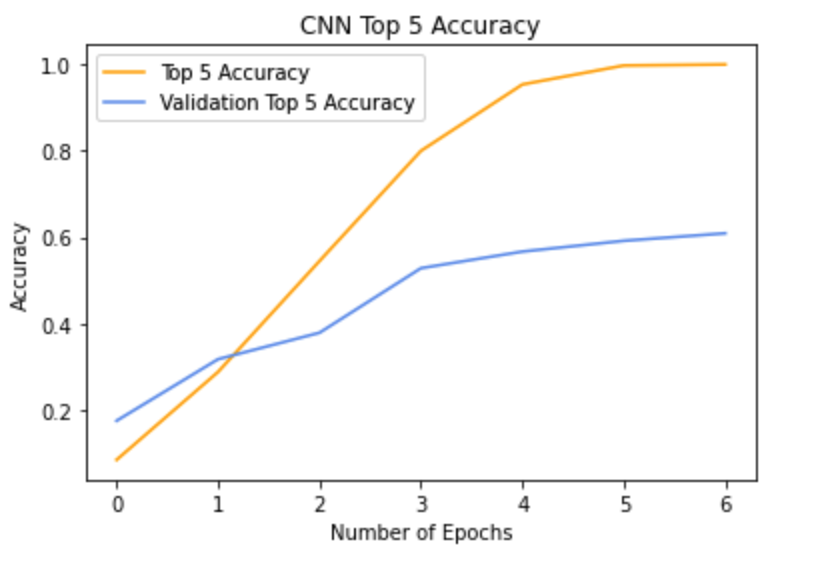
\includegraphics[width=0.5\textwidth]{images/cnntop5.png}
    \caption{Tuned CNN Top 5 Accuracy with Data Augmentation}
    \label{fig:top5cnn}
\end{figure}

On the whole, the model with the best result is as seen in Table \ref{tab:cnn_model}.

\begin{table}[!h]
  \begin{center}
    \caption{CNN Model}
    \label{tab:cnn_model}
    \begin{tabular}{l|c|r} % <-- Alignments: 1st column left, 2nd middle and 3rd right, with vertical lines in between
      \textbf{Layer} & \textbf{Output Shape} & \textbf{Params}\\
      \hline
      Conv2D & (None, 100, 100, 16) & 448 \\
      Conv2D & (None, 100, 100, 16) & 2320 \\
      MaxPooling2D & (None, 50, 50, 16) & 0\\
      BatchNormalization & (None, 50, 50, 16) & 64\\
      Dropout & (None, 50, 50, 16) & 0\\
      Conv2D & (None, 50, 50, 32) & 4640 \\
      Conv2D & (None, 50, 50, 32) & 9248 \\
      MaxPooling2D & (None, 25, 25, 32)  & 0\\
      Dropout & (None, 25, 25, 32) & 0\\
      Conv2D & (None, 25, 25, 64) & 18496 \\
      Conv2D & (None, 25, 25, 64) & 36928 \\
      MaxPooling2D & (None, 12, 12, 64) & 0\\
      BatchNormalization & (None, 12, 12, 64) & 256\\
      Dropout & (None, 12, 12, 64) & 0\\
      Flatten & (None, 9216) & 0 \\
      Dense & (None, 480) & 4424160 \\
      BatchNormalization & (None, 480) & 1920\\
      Dense & (None, 4251) & 2044731 \\
    \end{tabular}
      \small
      \item Trainable params: 6,542,091
  \end{center}
\end{table}

\subsubsection{Model 2}

The second model we utilized for classification leveraged transfer learning. There aren't an abundance of available pre-trained models to be found, but a good option was VGG16. The architecture of VGG16 can be seen at \autoref{fig:VGG16}.

\begin{figure}[!h]
    \centering
    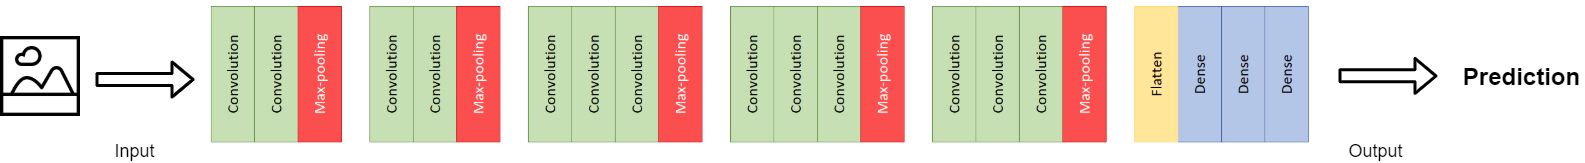
\includegraphics[width=1\textwidth]{VGG16.png}
    \caption{Architecture of VGG16}
    \label{fig:VGG16}
\end{figure}

Of note, the base VGG16 model has over 14 million trainable parameters. In order to leverage this model, we loaded weights that were trained on the ImageNet dataset, but replaced the final ImageNet classification layer with a maxpooling layer that belongs to the Feature Learning part of the network. The base model was then connected to a dropout layer (20\% drop chance), a dense fully connected layer (128 neurons), another dropout layer (20\% drop chance), and finally a dense fully connected layer used for classification on the whale dataset. 

It became immediately obvious that not just the imbalance of the dataset would be a problem, but also its size. We had intended to augment the under-represented samples, but this created a final output layer with over 5000 neurons resulting in a prohibitively large number of trainable parameters. This is particularly relevant due to the fine-tuning phase of a transfer learning process, where you train the entire model with a small learning weight. Instead, a minimum threshold was used to train the model using whales who were represented by at least 20 samples. This reduced the final number of target classes to 59. The final model used is shown in \autoref{tab:table2}. Reducing the final layer to this smaller subset of whales, however, meant that the intended use of the Playground dataset as validation data was no longer possible. Instead, the filtered training dataset was split into training and validation sets with a 3:1 ratio after having combined the Playground dataset with the Competition dataset to create an augmented training dataset.

\begin{table}[!h]
  \begin{center}
    \caption{Transfer Learning Model}
    \label{tab:table2}
    \begin{tabular}{l|c|r} % <-- Alignments: 1st column left, 2nd middle and 3rd right, with vertical lines in between
      \textbf{Layer} & \textbf{Output Shape} & \textbf{Params}\\
      \hline
      VGG16 & (512) & 14714688 (\textit{frozen})\\
      Dropout & (512) & 0\\
      Dense & (128) & 65664\\
      Dropout & (128) & 0\\
      Dense & (59) & 7611\\
    \end{tabular}
      \small
      \item Trainable params: 73,275
  \end{center}
\end{table}

With the base model's weights frozen, after training for 30 epochs the accuracy remained very low, not even reaching 40\%. The secret to good transfer learning, however, is by first training the weights of a novel classification layer with the pre-trained weights from the larger dataset, but then crucially, training the entire model with a small learning weight. In this fashion, you can leverage the pre-trained weights to relatively quickly set the new classification layer's weights to reasonable values. Then, the entire network is slowly updated with a small learning rate - this phase is called the fine-tuning phase. This transfer learning method typically results in a higher accuracy than even if the entire model was trained from scratch on only this small dataset. The entire model was trained for a further 30 epochs with a learning rate of 0.00001. The accuracy, and loss over time are shown in figures \autoref{fig:TLACC}, and \autoref{fig:TLLOSS} respectively. The final accuracy achieved was 90.28\%.

\begin{figure}[!h]
    \centering
    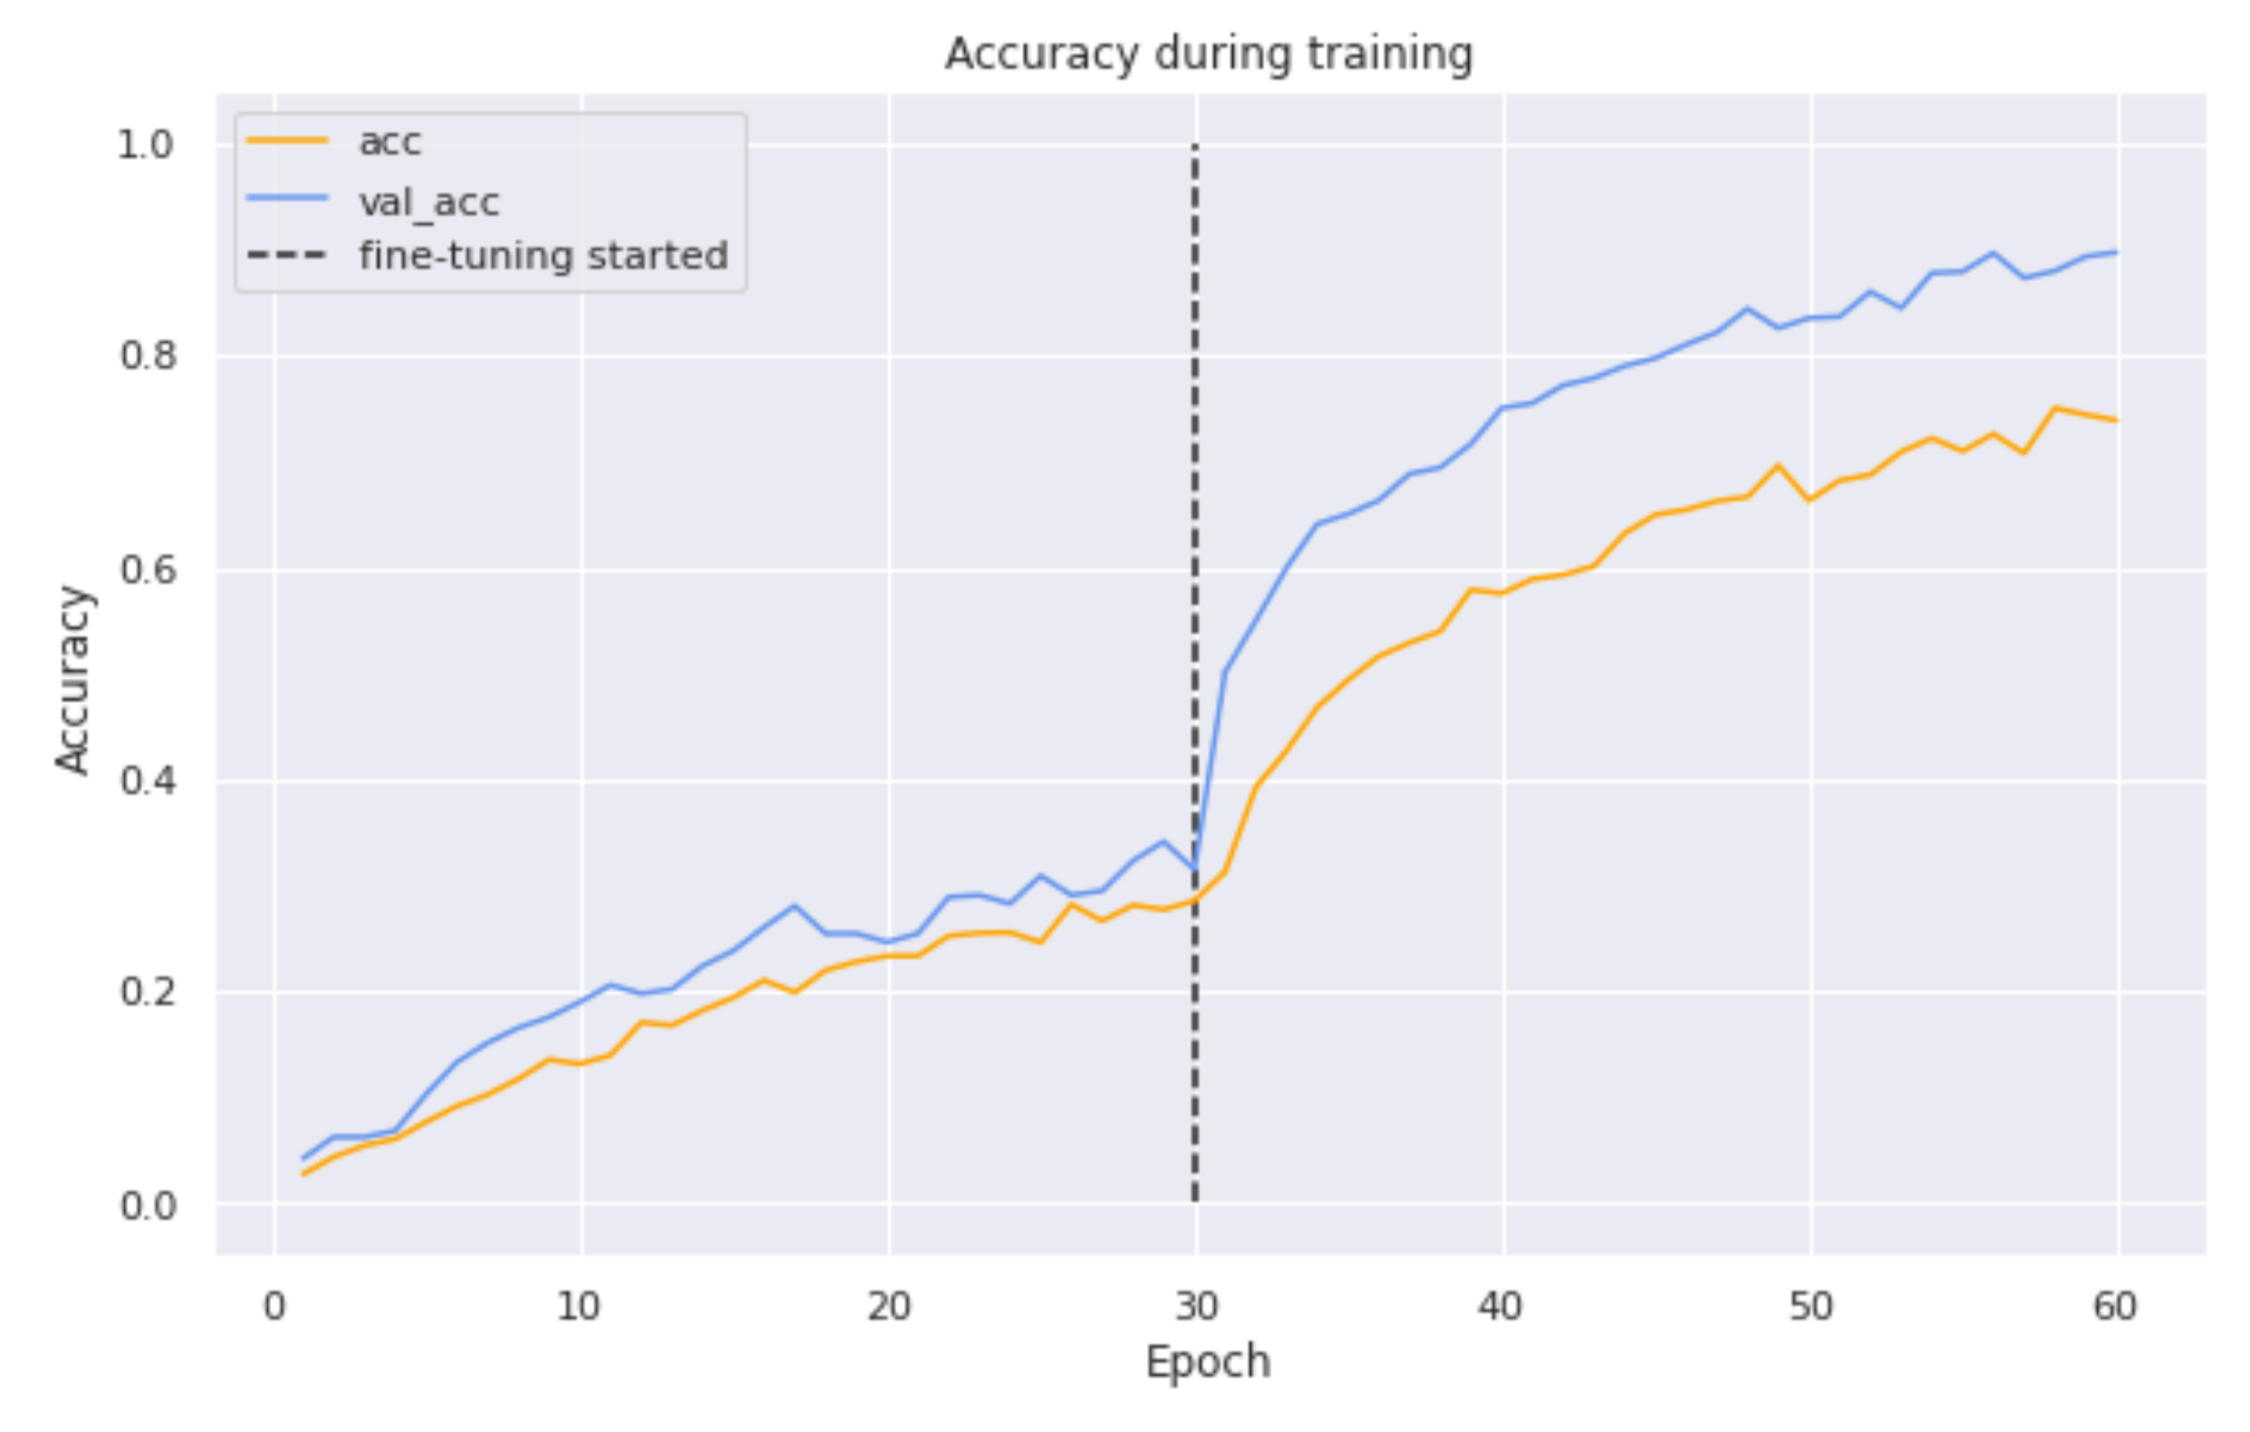
\includegraphics[width=0.5\textwidth]{TLaccuracy.png}
    \caption{VGG16 with whale instances of 20+ - Accuracy}
    \label{fig:TLACC}
\end{figure}

\begin{figure}[!h]
    \centering
    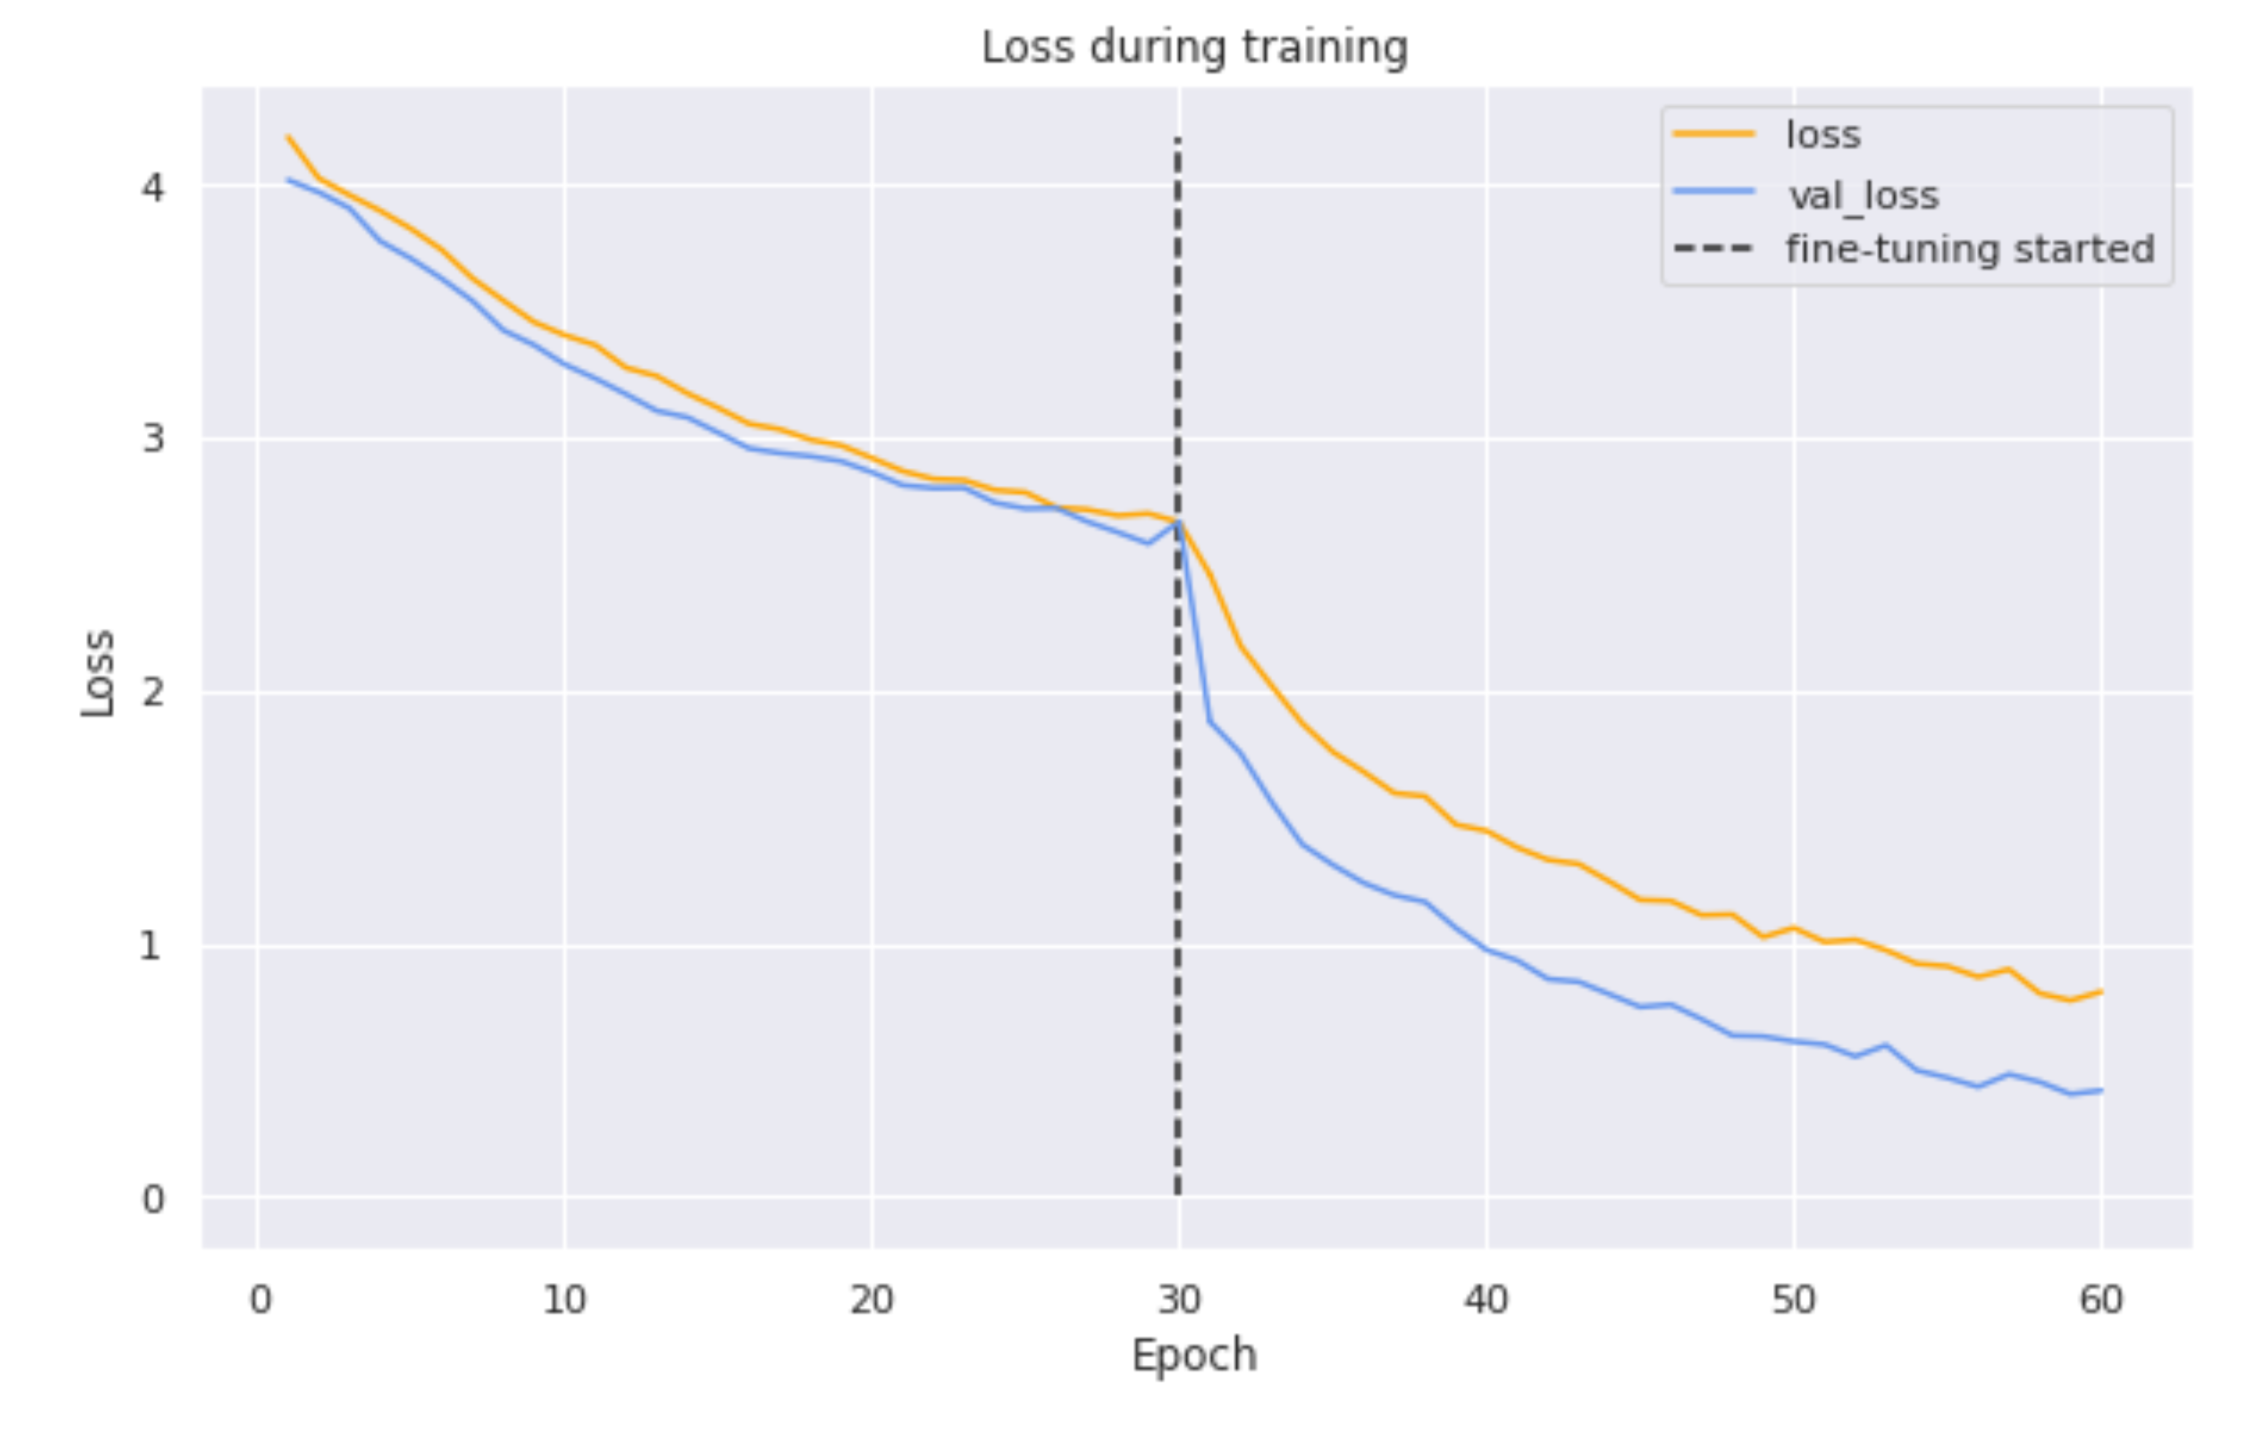
\includegraphics[width=0.5\textwidth]{TLloss.png}
    \caption{VGG16 with whale instances of 20+ - Loss}
    \label{fig:TLLOSS}
\end{figure}

We believe this model that leverages transfer learning could be improved further. Instead of reducing the training set rather arbitrarily to 59 classes (whales with at least 20 samples), the under-represented samples could instead be augmented and  included in the training dataset. While this model has the potential to score well on a test submission, it was only trained on 59 of the over 5000 provided unique whales. Obviously, it will not be able to identify the vast majority of whales - it is simply adept at classifying the whales it happened to be trained on. Training for such a complex model, however, would take a \textit{significant} period of time using a complex model such as VGG16.

With these potential increased benefits in mind, we determined that the maximum size of the dataset that we could train before running out of memory was by including all whales that had 5 or greater samples present. This increased the total possible output classifications of the model from 59 to 633 - creating a much more useful model. Additionally, since the actual competition was attempting to maximize a Top 5 Accuracy, we reattempted the Transfer Learning model to further improve our results while including the Top 5 Accuracy. After increasing the dataset to whales that had at least 5 samples, removing the erroneous data augmentation techniques as discussed in \autoref{subsec:Augmentation}, and by continuing to train until the model no longer improved, we obtained much better results. The top 5 accuracy, accuracy, and loss over time are shown in figures \autoref{fig:TLTOP5ACC5}, \autoref{fig:TLACC5}, and \autoref{fig:TLLOSS5} respectively. We achieved a final accuracy of 98.18\% and a final top 5 accuracy of 99.80\%.

\begin{figure}[!h]
    \centering
    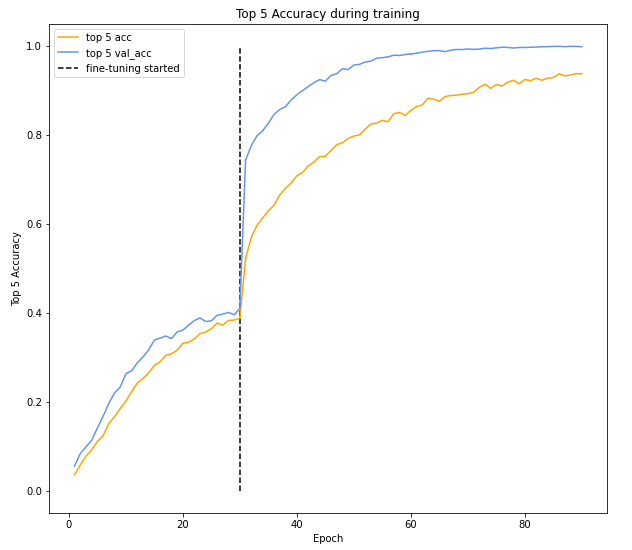
\includegraphics[width=0.5\textwidth]{TLtop5acc_big.png}
    \caption{VGG16 with whale instances of 5+ - Top 5 Accuracy}
    \label{fig:TLTOP5ACC5}
\end{figure}

\begin{figure}[!h]
    \centering
    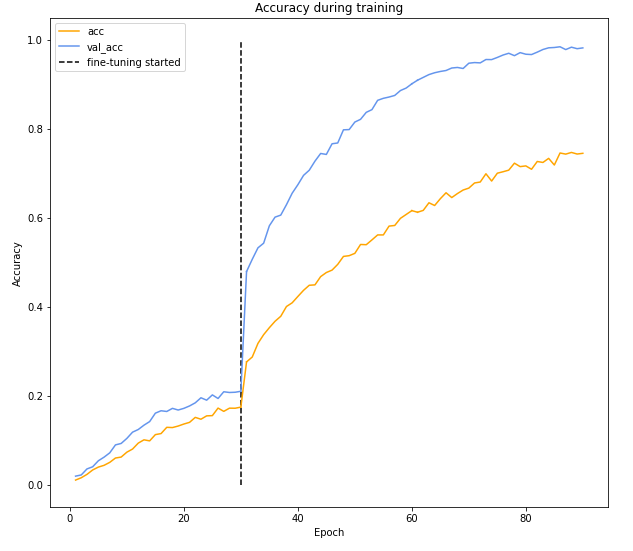
\includegraphics[width=0.5\textwidth]{TLaccuracy_big.png}
    \caption{VGG16 with whale instances of 5+ - Accuracy}
    \label{fig:TLACC5}
\end{figure}

\begin{figure}[!h]
    \centering
    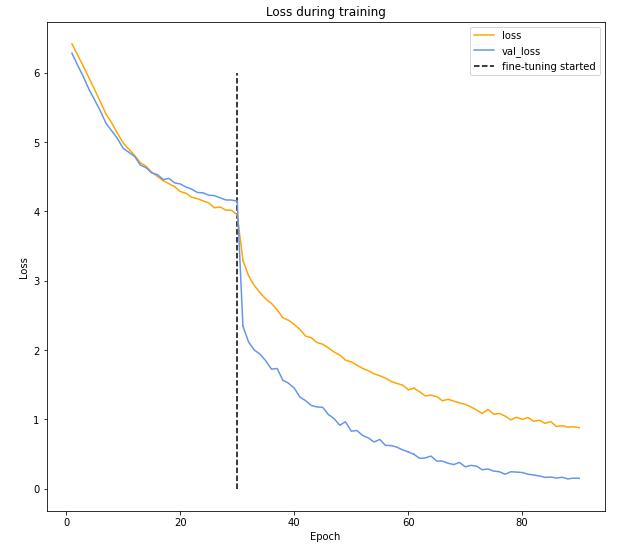
\includegraphics[width=0.5\textwidth]{TLloss_big.png}
    \caption{VGG16 with whale instances of 5+ - Loss}
    \label{fig:TLLOSS5}
\end{figure}

\pagebreak
\subsubsection {Model 3}
The third model utilized is the Support Vector Machine (SVM). It can easily handle multiple continuous and categorical variables. SVM constructs a hyperplane in multidimensional space to separate different classes. SVM generates optimal hyperplanes in an iterative manner, which is used to minimize an error. We did Data Augmentation here so that we can create additional data in the memory. As the data is large it will be better to use datagenerator, keras Imagedatagenerator was utilized. 

To convert NASNET into SVM; there is a parameter called “kernel regularizer” and inside this regularizer, l1 or l2 norm could be utilized. Here the l2 norm was used, linear activation function was employed in the final output layer in the model creation section. When a Support Vector Machine is used for binary classification LinearSVM is used. Linear SVM means a line is drawn between them which try to find out other margin lines and then divide the particular classes. Since this is a Multi-class Classification problem,  "squared hinge" is used as the loss function and softmax as the activation function during compiling for SVM. For the training set, 804 validated whales images belong to 28 classes and 268 validated images belong to 28 classes in the test set. SVM does not perform very well with this dataset, it gives a low validation accuracy. Other deep learning architecture such as the CNN or Transfer Learning used in this project or even You Only Look Once (YOLO) - a model used for real-time object detection - can serve as a base model for SVM required for further training.

\begin{figure}[!h]
    \centering
    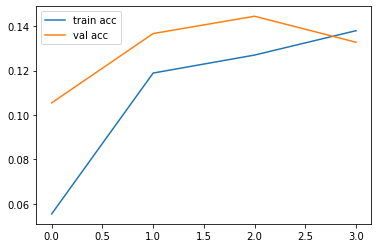
\includegraphics[width=0.5\textwidth]{svm_train_val_acc.png}
    \caption{SVM train and validation accuracy}
    \label{fig:TLLOSS5}
\end{figure}

\begin{figure}[!h]
    \centering
    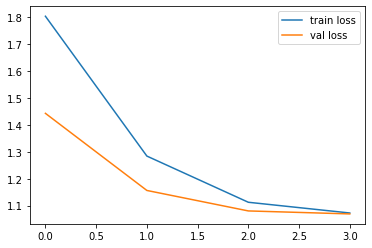
\includegraphics[width=0.5\textwidth]{svm_train_val_loss.png}
    \caption{SVM train and validation loss}
    \label{fig:TLLOSS5}
\end{figure}



\section{Experiment Results}\label{sec: experiment}
Our experiment utilized a couple of preprocessing and data augmentation techniques as mentioned above. Only 663 whales are represented in the dataset more than 5 times, 227 whales more than 10 times, while over 2,000 whales are represented by only a single sample. Due to this relatively small dataset size, data augmentation was necessary for reducing overfitting. The data prepossessing includes the removal of noise, cropping of images to show only the fluke, we performed data augmentation by flipping, rotating, and scaling the under-represented whale Id images. However, like in the case of Transfer Learning, some of the data augmentation processes also destroyed some of the features of the original images. By adjusting the augmentation done in the Transfer Learning model we were able to still utilize it to reduce overfitting while not destroying anything significant. We also ensured that while the CNN did not have the same issues as transfer learning with the augmentation, we used the same augmenting techniques for equal comparison. We also attempted to use traditional methods such as SVM. On the whole, CNN and Transfer Learning performed well in the whale identification task while SVM was not suitable for the problem. It is also clear that Transfer Learning outperforms CNN in this instance, especially with the processing constraints we were operating under. We can see the comparison of these results in Table \ref{tab:results}. It is clear that while CNN could work it needs more data and processing power to beat the Transfer Learning model.

\begin{table}[!h]
  \begin{center}
    \caption{Transfer Learning Model}
    \label{tab:results}
    \begin{tabular}{l|c|c|c|c}
      \textbf{Model} & \textbf{Train Acc} & \textbf{Val Acc} & \textbf{Top 5 Acc} & \textbf{Val Top 5 Acc} \\
      \hline
      CNN (5+ instances) & 0.999 & 0.420 & 0.999 & 0.615\\
      TL (5+ instances) & 0.745 & 0.981 & 0.937 & 0.998\\
      SVM (30+ instances) & 0.34 & 0.28 & 0.19&0.14\\
    \end{tabular}
  \end{center}
\end{table}

\section{Conclusion}\label{sec: conclusion}
Architecture such as the Transfer Learning or CNN done in this project clearly works well for tasks such as this. However, it is clear that in order for the CNN to truly compete with the transfer learning model, we would need more data and more processing power than we have access to in order to reduce the overfitting. SVM is also very clearly not the method to be used in this instance if deep learning models are available. In the future it would be interesting to see You Only Look Once (YOLO) architecture be utilized which uses high dimensional features as input to a deep neural network.

 
\needspace{20em}% Require at least 6em on the page
\newpage
\section{Team Contribution}\label{sec: teamcontribution}
See Table \ref{tab:contributionTable} for the breakdown of work and percentages.
\begin{table}[h!]
  \begin{center}
    \caption{Team Contribution}
    \label{tab:contributionTable}
    \begin{tabular}{l|l|c}
      \textbf{Team Member} & \textbf{Tasks Completed} & \textbf{Percentage of Project}\\
      \hline
      Stephen McKeon & \underline{Report}&  10\%\\
                     & ..Data Preprocessing &\\
                     & ..Data Augmentation &\\
                     & ..Model 2 &\\
                     & \underline{Data Preprocessing}& 7.5\%\\
                     & ..Bounding Box model&\\
                     & ..Crop, Affine Trans, Grey &\\
                     & \underline{Model 2 - Transfer Learning}& 15\%\\
      Emily Medema   & \underline{Report}& 10\%\\
                     & ..Abstract&\\
                     & ..Introduction&\\
                     & ..Background&\\
                     & ..Design&\\
                     & ..Methodology&\\
                     & ..Model 1&\\
                     & ..Experiment &\\
                     & ..Conclusion &\\
                     & \underline{Model 1 - CNN}& 15\%\\
                     & ..Data Preprocessing&\\
                     & \underline{Team Lead / Organizer}& 7.5\%\\
      Flourish Adebayo & \underline{Report}& 10\%\\
                     & ..Introduction&\\
                     & ..Background&\\
                     & ..Architecture Diagram&\\
                     & ..Model 3&\\
                     & ..Experiment&\\
                     & ..Conclusion&\\
                     & ..Bibliography&\\
                     & \underline{Presentation}& 10\%\\
                     & \underline{Model 3 - SVM}& 15\%\\
                     & ..Data Augmentation&\\          
    \end{tabular}
  \end{center}
\end{table}

\clearpage
\bibliography{references} 
\bibliographystyle{ieeetr}



%%% End document
\end{document}